\section{Regularization}
blau1
When dealing with many candidates to use as covariates, one has to deal with the problem of selecting a subset of variables to use in constructing the model. 
This means that the vector of coefficients $\beta_\alpha = [ \beta_{1 \alpha} \cdots \beta_{P\alpha} ]$ should not have all nonzero values.
There are many ways of selecting a subset of variables among.
A classic approaches for this problem is the Stepwise algorithm \cite{efroymson1960multiple}, which includes variables in sequence. 

The approach we use in  of doing regularization and selecting the best model for estimating the quantile function. At first, we use a Mixed Integer Linear Programming optimization problem (MILP) to find the best subset among all choices of covariates. The second way is by using a LASSO-type technique, which consists in penalizing the $\ell_1$-norm of regressors, thus shrinking the size of estimated coefficients towards zero.  

\subsection{Best subset selection with MILP}
\label{sec:best-subset-mip}

In this part, we investigate the usage of MILP to select which variables are included in the model, up to a limit of inclusions imposed \textit{a priori}. We establish that only $K$ coefficients $\beta_{p\alpha}$ may have nonzero values, for each quantile $\alpha$. 
This assumption is modeled with binary variables $z_{p\alpha}$, which indicates whether $\beta_{p\alpha}$ is included or not.
The optimization problem that incorporates this idea is described below:
\begin{eqnarray}
 \underset{\beta_{0\alpha},\beta_\alpha,z_{p \alpha} \varepsilon_{t \alpha}^{+},\varepsilon_{t \alpha}^{-}}{\text{min}} & \sum_{\alpha \in A} \sum_{t\in T}\left(\alpha\varepsilon_{t \alpha}^{+}+(1-\alpha)\varepsilon_{t\alpha}^{-}\right) \label{eq:mip0} \\
\mbox{s.t } & \varepsilon_{t \alpha}^{+}-\varepsilon_{t \alpha}^{-}=y_{t}-\beta_{0 \alpha}-\sum_{p=1}^{P}\beta_{p \alpha}x_{t,p},& \qquad\forall t \in T ,\forall \alpha \in A, \label{eq:mip1}\\
& \varepsilon_{t \alpha}^{+},\varepsilon_{t \alpha}^{-}\geq0,&\qquad\forall t \in T ,\forall \alpha \in A, \label{eq:mip2}\\
& - M z_{p \alpha} \leq \beta_{p \alpha} \leq M z_{p \alpha},&\qquad\forall p\in\{1,\dots,P\}, \label{eq:mip3}\\
& \sum_{p=1}^P z_{p \alpha} \leq K, & \qquad \forall \alpha \in A, \label{eq:mip4}\\
& z_{p \alpha} \in \{0,1\},&\qquad\forall p\in\{1,\dots,P\}, \forall \alpha \in A, \label{eq:mip5}\\
& \beta_{0\alpha} + \beta_{\alpha}^T x_{t} \leq \beta_{0\alpha'} + \beta_{\alpha'}^T x_{t}, & \qquad \forall t \in T, \forall (\alpha, \alpha') \in A \times A,  \alpha < \alpha',\nonumber\\ \label{eq:mip6}
\end{eqnarray}
The objective function and constraints (\ref{eq:mip1}), (\ref{eq:mip2}) and (\ref{eq:mip6}) are those from the standard linear quantile regression. 
By constraint (\ref{eq:mip3}), variable $z_{p \alpha}$ is a binary that assumes 1 when the coefficient $\beta_{p \alpha}$ is included, while (\ref{eq:mip4}) guarantees that  


The other constraints implement the process of regularization, forcing a maximum of $K$ variables to be included in the model. 


$M$ is chosen in order to guarantee that $M \geq \|\hat{\beta_\alpha}\|_{\infty}$. The solution given by $\beta_{0\alpha}^*$ and $\beta_\alpha^* = [ \beta_{1 \alpha}^* \cdots \beta_{P\alpha}^* ]$ will be the best linear $\alpha$-quantile regression with $K$ nonzero coefficients. 

{
	\def\OldComma{,}
	\catcode`\,=13
	\def,{%
		\ifmmode%
		\OldComma\discretionary{}{}{}%
		\else%
		\OldComma%
		\fi%
	}%
	We ran this optimization on the Icaraizinho dataset for each value of $K \in \{0, 1, \dots, 12\}$ and quantiles $\alpha \in \{0.05, 0.1, 0.5, 0.9, 0.95\}$. The full results table can be accessed on section \ref{sec:mipcoefficients}. For all quantiles the 12\textsuperscript{th} lag was the one included when $K=1$. When $K=2$, the 1\textsuperscript{st} lag was always included, sometimes with $\beta_{12}$, some others with $\beta_4$ and once with $\beta_{11}$. These 4 lags that were present until now are the only ones selected when $K=3$. For $K=4$, those same four lags were selected for three quantiles (0.05, 0.1 and 0.5), but for the others (0.9 and 0.95) we have $\beta_6$, $\beta_7$ and $\beta_9$ also as selected. From now on, the inclusion of more lags represent a lower increase in the fit of the quantile regression. The estimated coefficient values for all $K$'s are available in the appendices section. 
}

\subsubsection*{Defining groups for variables}

Consider the optimization problem defined on (\ref{eq:mip0})-(\ref{eq:mip6}). Equation (\ref{eq:mip3}) permits a different subset for each $\alpha$-quantile, whose function is defined by a set of $K$ variables. For two similar probabilities $\alpha$ and $\alpha'$, it is not plausible that their chosen model be too different (for example, for the $\alpha$ quantile one selects $\beta_{1\alpha}$ and $\beta_{4\alpha}$ and for the $\alpha'$ quantile one selects $\beta_{2\alpha}$ and $\beta_{5\alpha}$), which is allowed by the previous optimization model.

To address this issue, we propose to divide all $\alpha \in A$ into groups. The collection $G$ of all groups $g$ form a partition of $A$, and each $\alpha$ will belong to exactly one group $g$. 
The subset of selected covariates must be the same for all $\alpha$ in the same group $g$. To model these properties as constraints, we use the following equations and inequalities, that take the place of inequality \ref{eq:mip3} on the optimization problem:
\begin{eqnarray}
&z_{p \alpha} := 2 - ( 1-z_{pg}) - I_{g\alpha}& \\
& \sum\limits_{g \in G} I_{g\alpha} = 1, & \forall \alpha \in A,\label{eq:mipgrupa} \\
& -Mz_{p \alpha}  \leq  \beta_{p \alpha} \leq M z_{p \alpha}, & \forall p \in P, \quad \forall \alpha \in A, \quad \forall g \in G, \label{eq:mipgrupb} \\
& I_{g\alpha}, z_{pg} \in \{0,1\},& \forall p \in P, \quad \forall g \in G, 
\end{eqnarray}
where $G$ is a set of group index and $z_{pg}$ is a binary variable that equals 1 iff covariate $p$ is included on group $g$ and $I_{g\alpha}$ equals 1 iff $\alpha$ belongs to group $g$.
The logic behind constraint \ref{eq:mipgrupb} is that 
$$\text{If }z_{pg} = 0 \text{ and }I_{g\alpha} =1 \text{ then } \beta_{p \alpha = 0}. $$
Note that variable $z_{p \alpha}$ behaves differently that when we are not considering groups
This means that if probability $\alpha$ belongs to group $g$ but variable $p$ is not selected to be among


\subsection{Best subset selection with a $\ell_1$ penalty}
\label{sec:best-subset-ell1}

Another way of doing regularization is including the $\ell_1$-norm of the coefficients on the objective function. The advantage of this method is that coefficients are shrunk towards zero, and only some of them will have nonzero coefficients. The lower the imposed penalty ($\lambda$) on the $\ell_1$-norm, more variables are included in the model. 
This is the same strategy of the LASSO methodology, and its usage for the quantile regression is discussed in \cite{li2012l1}.
The proposed optimization problem to be solved is:
\begin{equation}
\underset{\beta_{0\alpha},\beta_\alpha}{\text{min}} \sum_{t \in T}\alpha|y_{t}-q_\alpha(x_t)|^{+}+ \sum_{t \in T}(1-\alpha)|y_{t}-q_\alpha(x_t)|^{-}+\lambda\|\beta_\alpha\|_{1}
\label{eq:l1-qar-optim}
\end{equation}
\[
q_\alpha(x_t)=\beta_{0}-\sum_{p=1}^{P}\beta_{p}x_{t,p},
\]
where the regressors $x_{t,p}$ used are its lags. In order to represent the above problem to be solved with linear programming solver, we restructure the problem as below:
\begin{eqnarray}
\beta_\lambda^{*LASSO} = \underset{\beta_{0},\beta,\varepsilon_{t \alpha}^{+},\varepsilon_{t \alpha}^{-}}{\text{arg min}} & \sum_{\alpha \in A} \sum_{t \in T}\left(\alpha\varepsilon_{t \alpha}^{+}+(1-\alpha)\varepsilon_{t \alpha}^{-}\right)+\lambda\sum_{p=1}^{P}\mbox{\ensuremath{\xi}}_{p} \label{eq:obj-lasso} \\
\mbox{s.t. } & \varepsilon_{t \alpha}^{+}-\varepsilon_{t \alpha}^{-}=y_{t}-\beta_{0}-\sum_{p=1}^{P}\beta_{p}x_{t,p},&\forall t\in T,\\
& \varepsilon_{t \alpha}^{+},\varepsilon_{t \alpha}^{-}\geq0,&\forall t \in T, \forall \alpha \in A\\
& \xi_{p}\geq\beta_{p \alpha},&\forall p\in\{1,\dots,P\}, \forall \alpha \in A  \nonumber\\ \label{l1-qar-3}
\\
& \xi_{p}\geq-\beta_{p \alpha},&\forall p\in\{1,\dots,P\}, \forall \alpha \in A,  \nonumber \\ \label{l1-qar-4}
\end{eqnarray}
This model is built upon the standard linear programming model for the quantile regression (equation \ref{eq:qar-lp}). 
On the above formulation, the $\ell_1$ norm of equation (\ref{eq:l1-qar-optim}) is substituted by the sum of $\xi_p$, which represents the absolute value of $\beta_p$. The link between variables $\xi_p$ and $\beta_p$ is made by constraints (\ref{l1-qar-3}) and (\ref{l1-qar-4}). Note that the linear coefficient $\beta_0$ is not included in the penalization, as the sum of penalties on the objective function \ref{eq:obj-lasso}.

For such estimation to produce good results, however, each variable must have the same relative weight in comparison with one another. So, before solving the optimization problem, we normalize all variables to have mean $\mu = 0$ and variance $\sigma^2 = 1$. For the vector of observations for each covariate (that in our problem represents is a vector of observations of lags $y_{t-p}$), we apply the transformation $\tilde{y}_{t-p,i} = (y_{t-p,i} - \bar{y}_{t-p}) / \sigma_{t-p}$, where $\bar{y}_{t-p}$ is the $p$-lag mean and $\sigma_{t-p}$ the $p$-lag standard deviation. We use the $\tilde{y}_{t-p,i}$ series to estimate the coefficients. Once done that, we multiply each coefficient for its standard deviation to get the correct coefficient: $\beta_i = \tilde{\beta}_i \sigma_{t-p}$.

For low values of $\lambda$, the penalty is small and thus we have a model where all coefficients have a nonzero value. On the other hand, while $\lambda$ is increased the coefficients shrink towards zero; in the limit we have a constant model. For instance, we don't penalize the linear coefficient $\beta_0$. For the same quantiles values $\alpha$ we experimented on section \ref{sec:best-subset-mip} ($\alpha \in \{0.05, 0.1, 0.5, 0.9, 0.95\}$). 

\begin{figure}
	\centering
	\begin{minipage}[t]{0.4\linewidth}
		\centering
		\begin{minipage}[t]{\linewidth}
			\centering     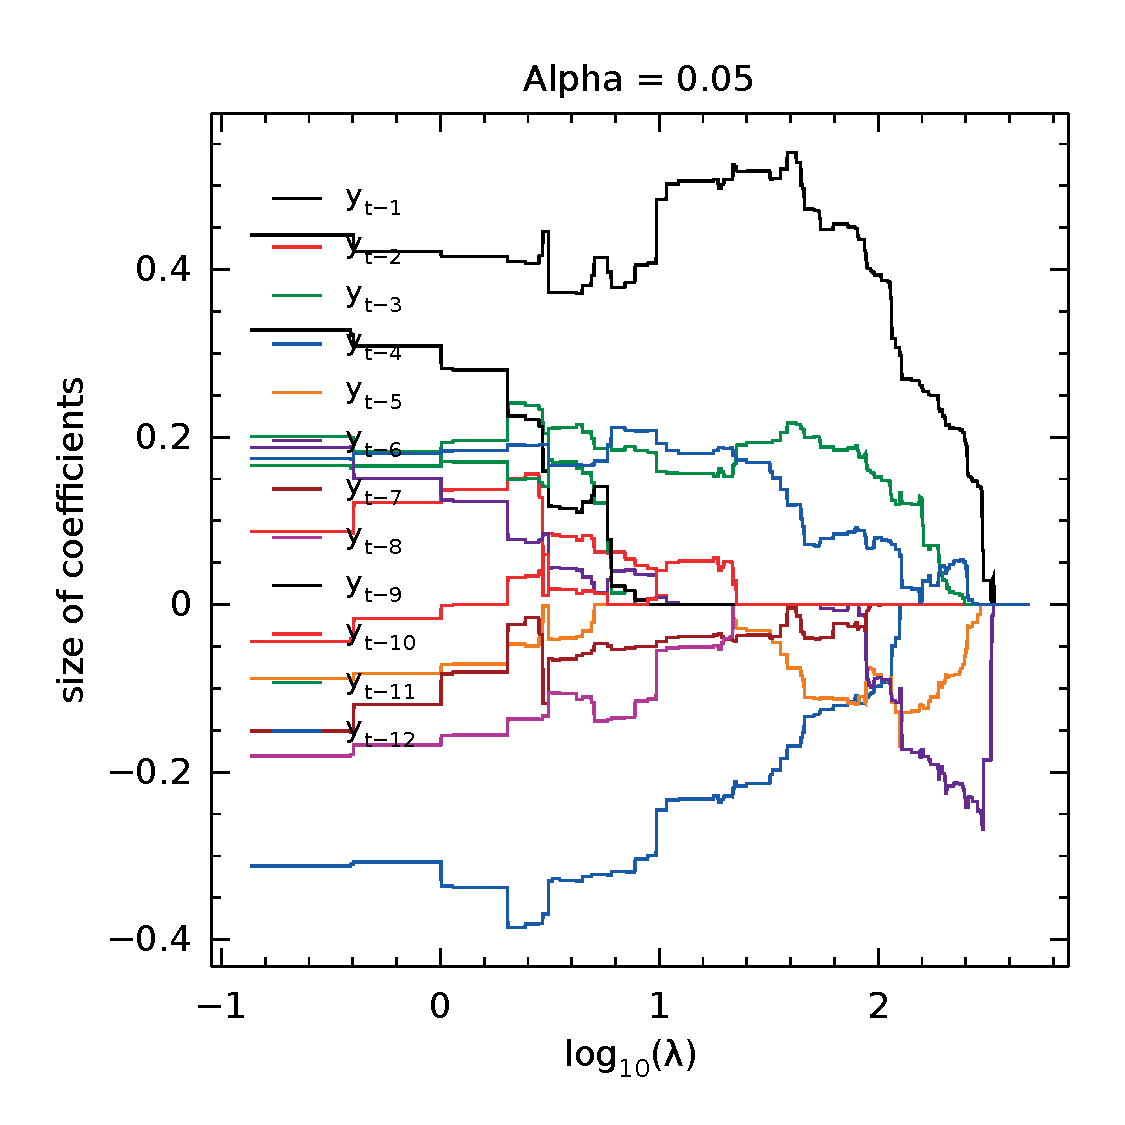
\includegraphics[width=\textwidth]{Figuras/selecao-lasso/par-sellasso-005.pdf}
		\end{minipage}
		\begin{minipage}[b]{\linewidth}
			\centering     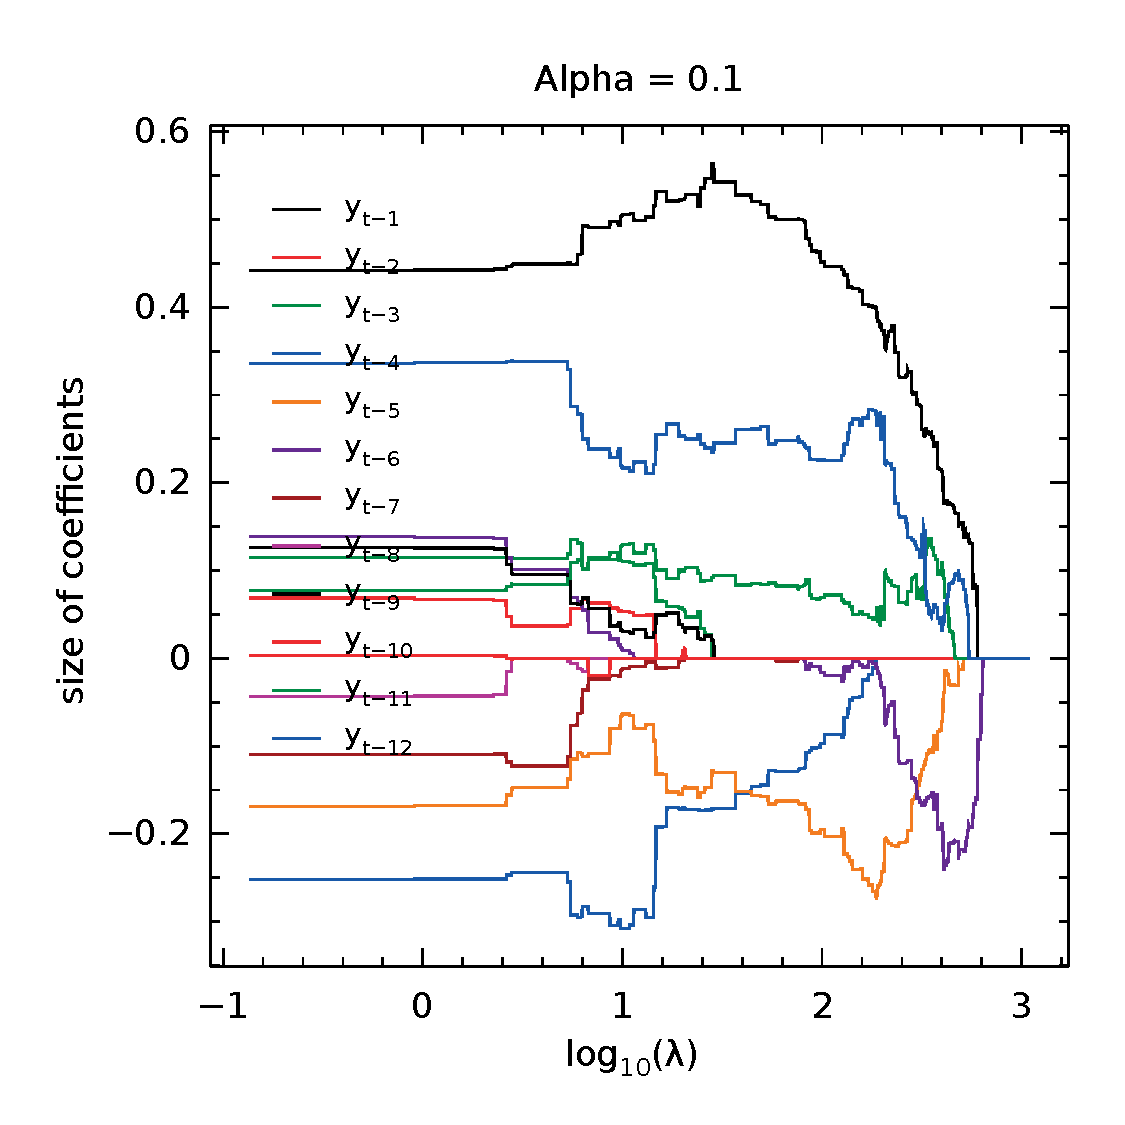
\includegraphics[width=\textwidth]{Figuras/selecao-lasso/par-sellasso-01.pdf}
		\end{minipage}
		\begin{minipage}[b]{\linewidth}
			\centering     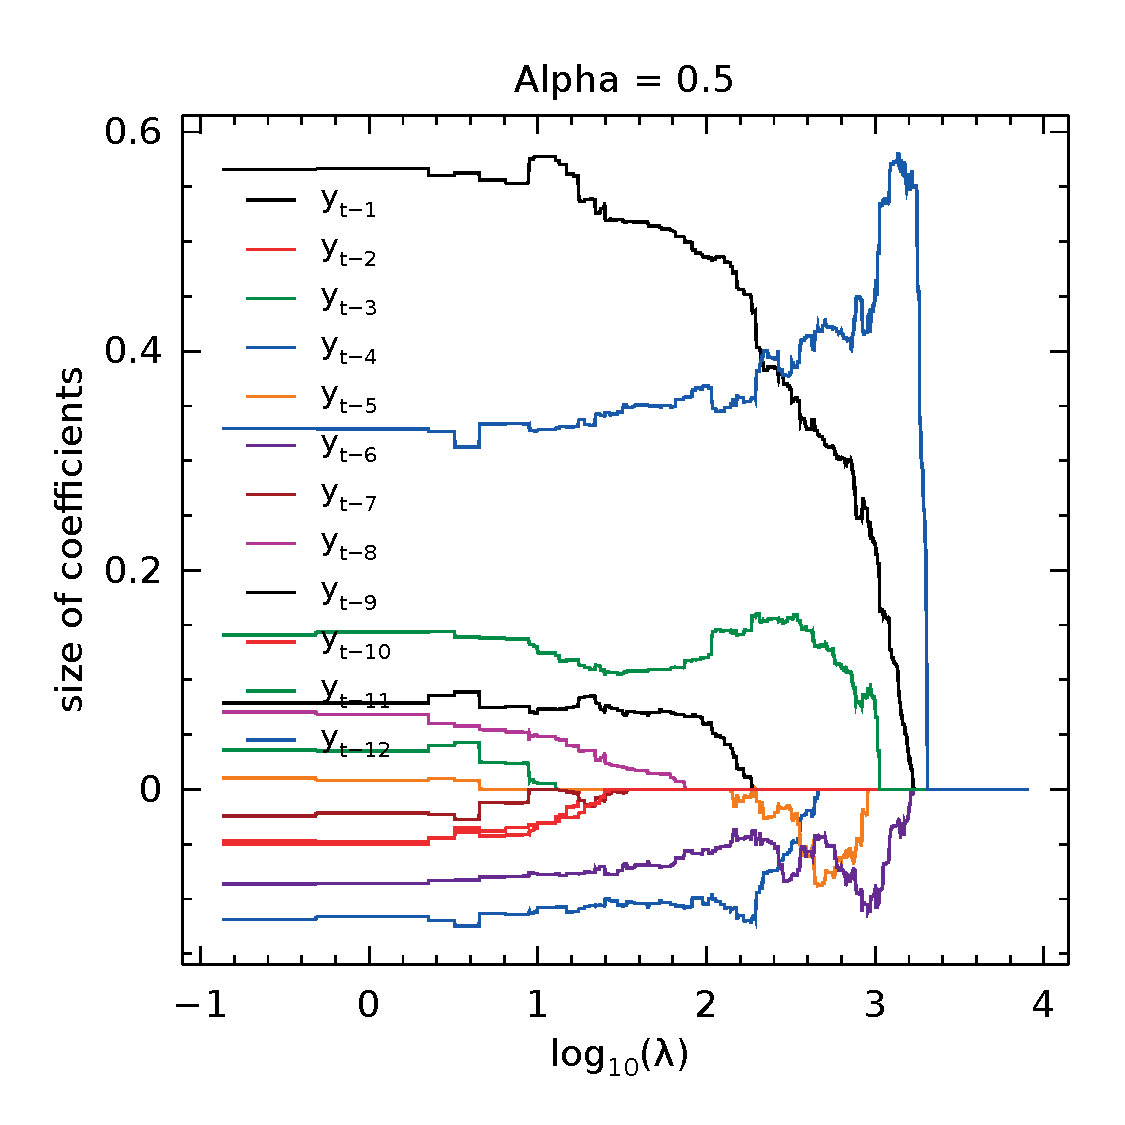
\includegraphics[width=\textwidth]{Figuras/selecao-lasso/par-sellasso-05.pdf}
		\end{minipage}
	\end{minipage}
	\begin{minipage}[t]{0.4\linewidth}
		\centering
		\begin{minipage}[b]{\linewidth}
			\centering     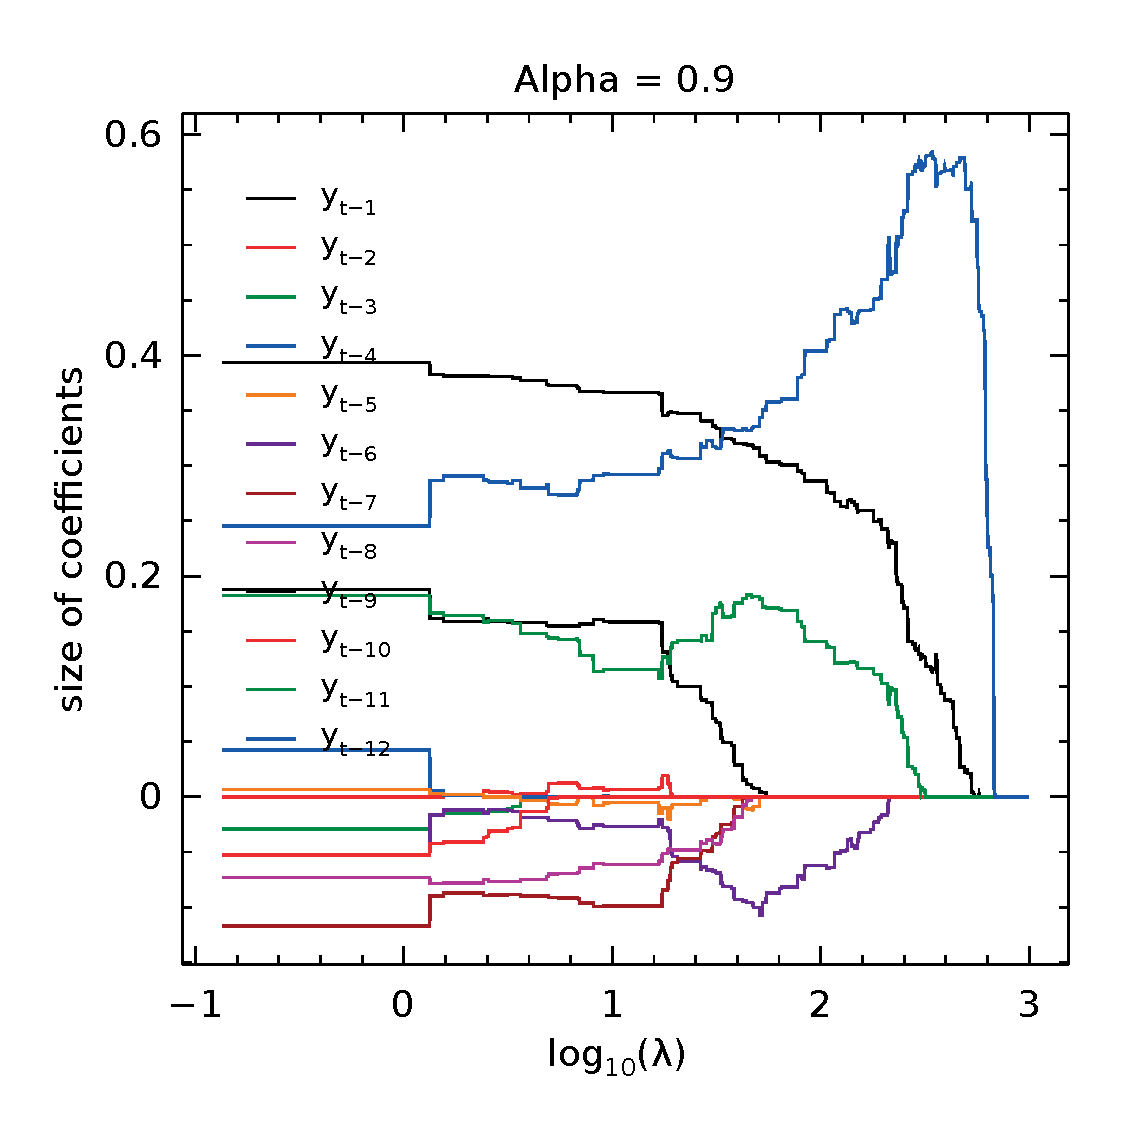
\includegraphics[width=\textwidth]{Figuras/selecao-lasso/par-sellasso-09.pdf}
		\end{minipage}
		\begin{minipage}[b]{\linewidth}
			\centering     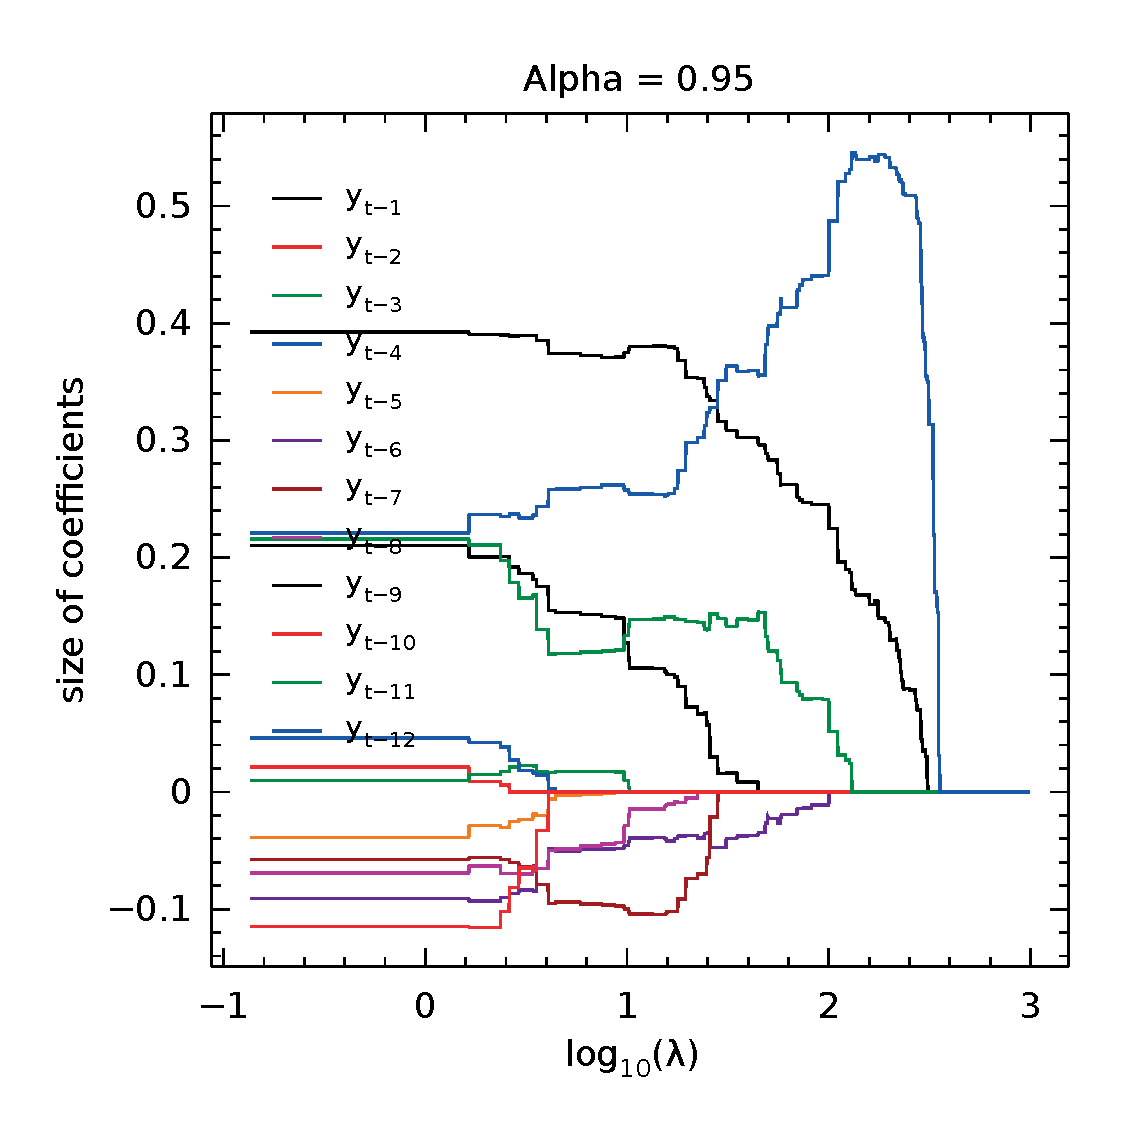
\includegraphics[width=\textwidth]{Figuras/selecao-lasso/par-sellasso-095.pdf}
			\label{fig:npqar-cross}
		\end{minipage}
	\end{minipage}
	\caption{Coefficients path for a few different values of $\alpha$-quantiles. $\lambda$ is presented in a $\log_{10}$ scale, to make visualization easier.}
	\label{fig:npqar-results}
\end{figure}

It is important to mention that even though we have coefficients that are estimated by this method, we don't use them directly. Instead, the nonzero coefficients will be the only covariates used as explanatory variables of a regular quantile autoregression, solved by the linear programming problem \ref{eq:qar-lp}. In summary, the optimization in equation \ref{eq:l1-qar-optim} acts as a variable selection for the subsequent estimation, which is normally called the post-LASSO estimation \cite{belloni2009least}.

In this estimation made \textit{a posteriori}, only a subset of the $P$ covariates will have nonzero values, which are given by the set 
\begin{equation*}
L_\lambda = \{ p \; | \; p \in \{ 1,\dots,P \}, \; |\beta^{*LASSO}_{\lambda,p}| \neq 0  \}.
\end{equation*}
Hence, we have that
$$\beta^{*LASSO}_{\lambda,p} = 0 \iff \beta^{*}_{\lambda,p} = 0.$$
The post-lasso coefficients $\beta_\lambda^*$ are the solution from the optimization problem given below:
\begin{equation}
\begin{aligned} (\hat{\sigma}_{\lambda}^{*},\beta_{\lambda}^{*})\overset{(obj,var)}{\longleftarrow} \min_{\beta_0,\beta,\varepsilon_{t}^{+},\varepsilon_{t}^{-}} & \sum_{t \in T}\left(\alpha\varepsilon_{t}^{+}+(1-\alpha)\varepsilon_{t}^{-}\right) \\
\mbox{s.t. } & \varepsilon_{t}^{+}-\varepsilon_{t}^{-}=y_{t} - \beta_0 - \sum_{p\in L_\lambda} \beta_p x_{t,p},& \forall t\in T,\\
& \varepsilon_t^+,\varepsilon_t^- \geq 0, & \forall t \in T.
\end{aligned}
\label{eq:post-lasso}
\end{equation}
The variable $\hat{\sigma}_{\lambda}^{*}$ receives the value of the objective function on its optimal solution.






\subsection{Model selection}

On sections \ref{sec:best-subset-mip} and \ref{sec:best-subset-ell1}, we presented two ways of doing regularization. Nonetheless, regularization can be done with different levels of parsimony. For example, one can select a different number $K$ of variables to be included in the best subset selection via MILP or choose different values of $\lambda$ for the $\ell_1$ penalty. Each of these choices may lead to a different model, and th ......... 

% % % Métrica

Solving a LP problem is much faster than a similar-sized MILP problem. One of our goals is to test whether a solution of a model with a $\ell_1$-norm can approximate well a solution given by the MILP problem. We propose an experiment that is described as follows. First, we calculate the quantity $\| \beta^*_\lambda \|_0$ of nonzero coefficients, for each given lambda, for the LASSO estimations.
Then, for each number $K$ of total nonzero coefficients, there will be a penalty $\lambda^*_K$ which minimizes the errors from the quantile regression's objective function (given on equation (\ref{eq:post-lasso})): 
\todo{($K$ ranging from 0 until 12, where 0 means that only the intercept is included)}

\begin{equation}
\lambda^*_K = \argmin_\lambda \left\lbrace \left.  \hat{\sigma}_{\lambda}^{*} \quad  \right| \, \| \beta^*_\lambda \|_0 = K \right\rbrace.
\end{equation}
We, then, define the set $L_K^{m}$, which contains all nonzero indexes, for a given $K$, of method $m$.
Thus, we can compare the best lasso fit where exactly $K$ variables are selected with the best fit given by the MILP problem, also with $K$ variables selected.

As the MILP solution is the exact solution for the problem, while the LASSO solution is an approximation, we use the former as a \textit{benchmarking} for the quality of the latter solution. To help us view the difference of results between both methods, we define a similarity metric $d$ between the subset of coefficients chosen by each one of them. It is desirable that the LASSO solution be as related with the MILP solution as possible.
The similarity is calculated as the solution of the following optimization problem
\begin{eqnarray}
d(\beta^*_{MILP(K)}, \beta^*_{\lambda^*_K}) =	1 - \max_{0\leq\delta_{ij}\leq1} & \sum\sum_{j} \delta_{ij} |\rho_{ij}| \label{eq:metricad0} \\
\text{s.t.} & \sum_{j}\delta_{ij}=1 & \forall i\in L_{K}^{MILP},\\
& \sum_{i}\delta_{ij}=1 & \forall j\in L_{K}^{LASSO},\\
& \delta_{i,j} = 0, & \forall i \in \overline{L}_{K}^{MILP}, \forall j \in \{1,\dots,P\},\\
& \delta_{i,j} = 0, & \forall j \in \overline{L}_{K}^{LASSO}, \forall i \in \{1,\dots,P\},\label{eq:metricad4}
\end{eqnarray}
where $\rho_{ij}$ is the correlation between variables $i$ and $j$ and $\delta_{ij} = 1$ means that the selected variable $i$ from the set $L_k^{MILP}$ is associated with the variable $j$ from set $L_k^{LASSO}$, and the constraints guarantee that each variable is related with only one other variable. The set $\overline{L}_K^{m}$ represents the variable indexes $\{1,\dots,P\} \backslash {L}_K^{m}$ for the method $m$ which are not present in ${L}_K^{m}$.
When $d = 0$, both solutions are equal, and the LASSO method was able to select the best subset among the available possibilities.
% % % Trocar o sigma da função objetivo.




% % % recolocar no texto
As seen before, we have a best solution for each desired $K$. The question that arises now is how to select the ideal number of variables to use.
One way of achieving this is by using an information criteria to guide our decision. 
An information criteria summarizes two aspects. One of them refers to how well the model fits the in-sample observations. The other part penalizes the quantity of covariates used in the model. By penalizing how big our model is, we prevent overfitting from happening. So, in order for a covariate to be included in the model, it must supply enough goodness of fit.
In \cite{machado1993robust}, it is presented a variation of the Schwarz criteria for M-estimators that includes quantile regression. The Schwarz Information Criteria (SIC), adapted to the quantile autoregression case, is presented below:
\begin{align} 
\begin{split}
SIC(m) = n \log(\hat{\sigma}^*)+\frac{1}{2}K\log n,\label{eq:SIC}
\end{split}					
\end{align}
where $K$ is the model's dimension. This procedure leads to a consistent model selection if the model is well specified. 

Figure \ref{fig:comparison-lm-results} shows the results of these experiments for quantiles $\alpha \in \{0.05, 0.1, 0.5, 0.9, 0.95\}$. The results point us that for small values of $K$ the distance between coefficients is bigger and where we observe the biggest differences between the SIC values. In this experiment, the minimum SIC value for the MILP problem is usually found between 4 and 6 variables in the model.

\begin{figure}
	\centering
	\begin{minipage}[t]{0.4\linewidth}
		\centering
		\begin{minipage}[t]{\linewidth}
			\centering     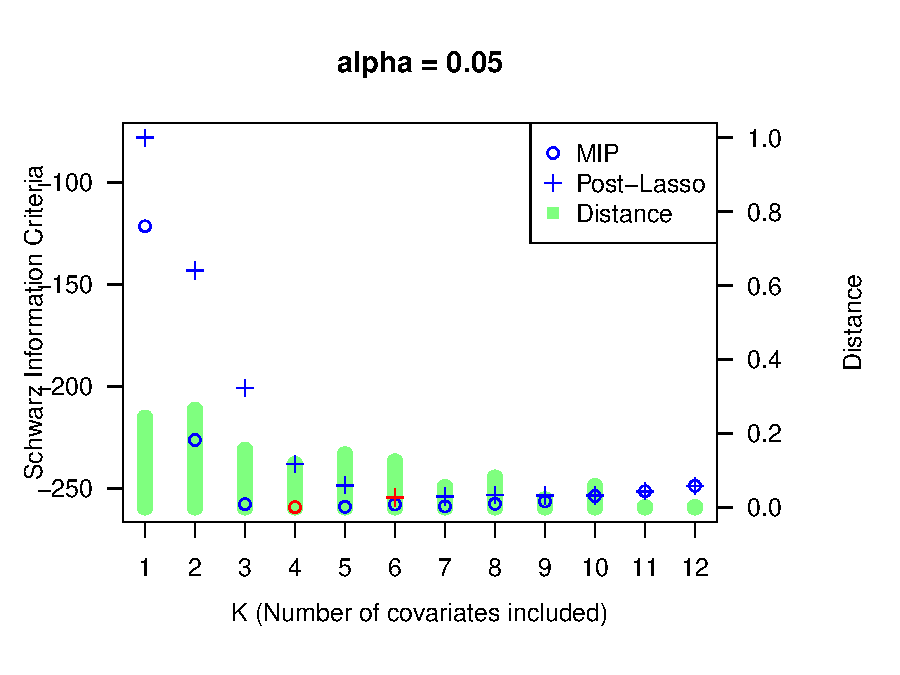
\includegraphics[width=\textwidth]{Figuras/SIC005.pdf}
		\end{minipage}
		\begin{minipage}[b]{\linewidth}
			\centering     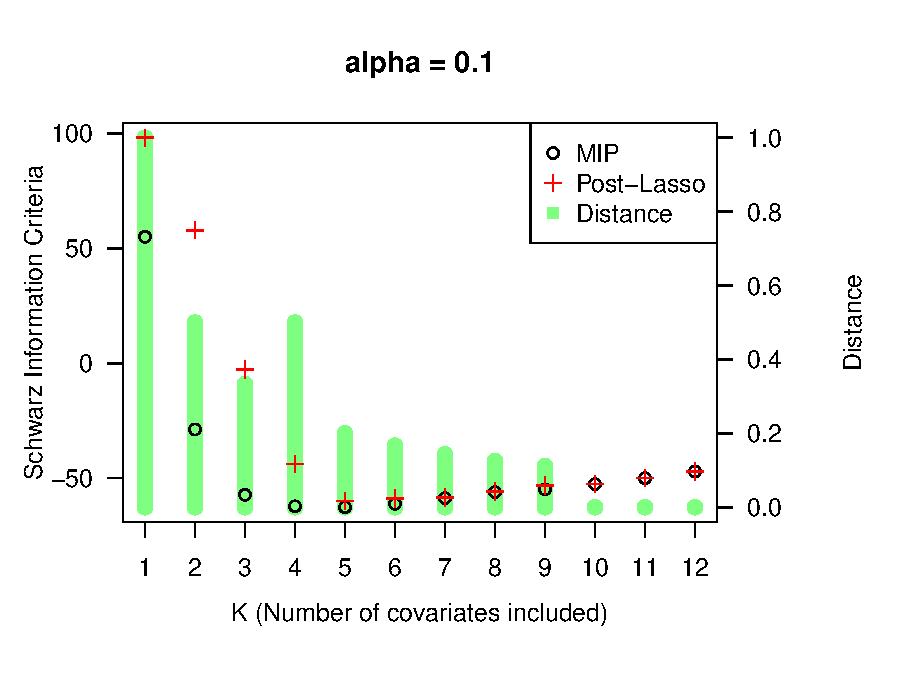
\includegraphics[width=\textwidth]{Figuras/SIC01.pdf}
		\end{minipage}
		\begin{minipage}[b]{\linewidth}
			\centering     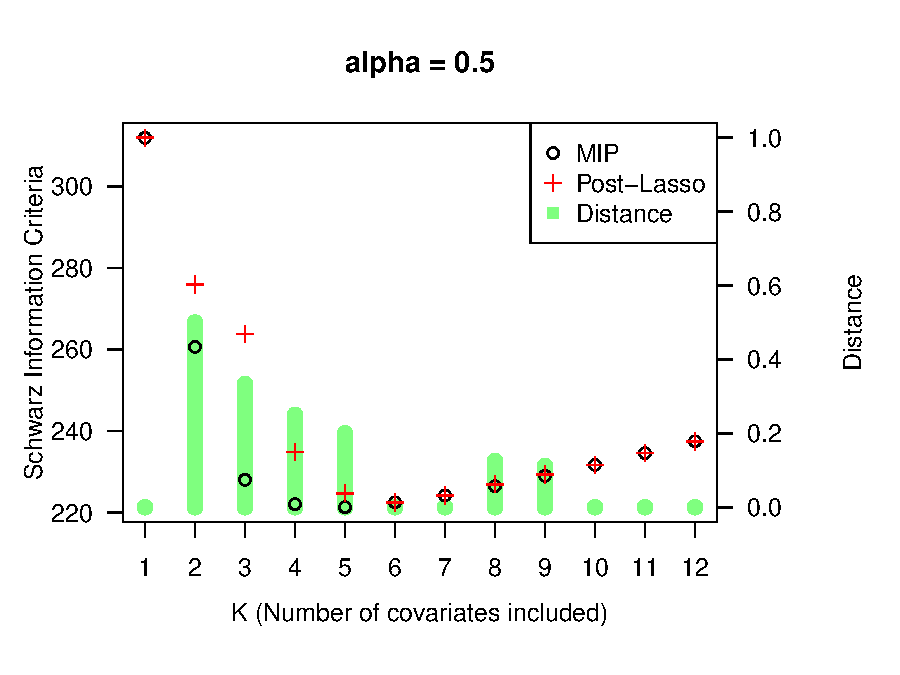
\includegraphics[width=\textwidth]{Figuras/SIC05.pdf}
		\end{minipage}
	\end{minipage}
	\begin{minipage}[t]{0.4\linewidth}
		\centering
		\begin{minipage}[b]{\linewidth}
			\centering     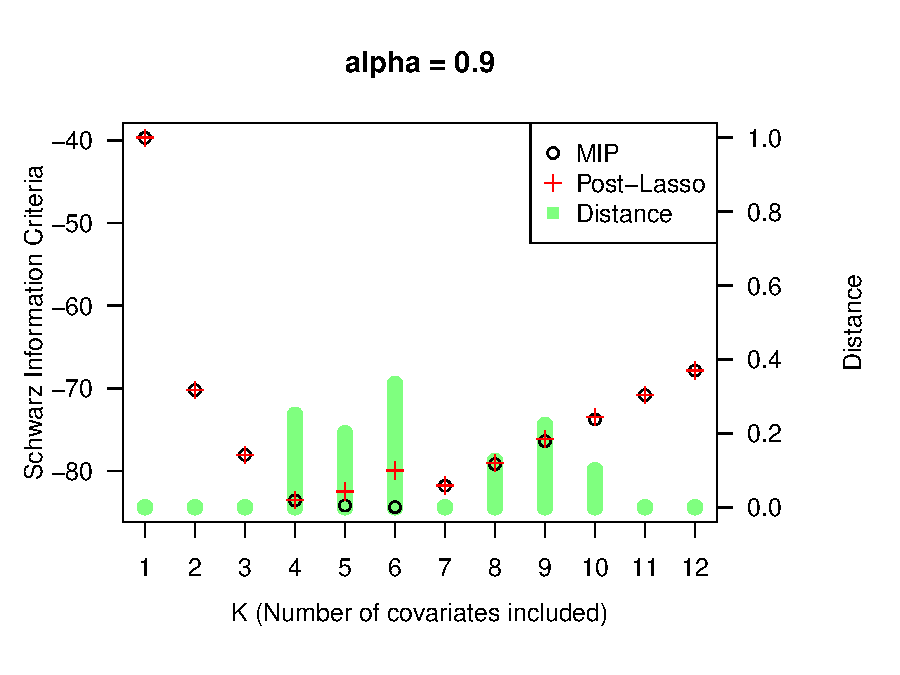
\includegraphics[width=\textwidth]{Figuras/SIC09.pdf}
		\end{minipage}
		\begin{minipage}[b]{\linewidth}
			\centering     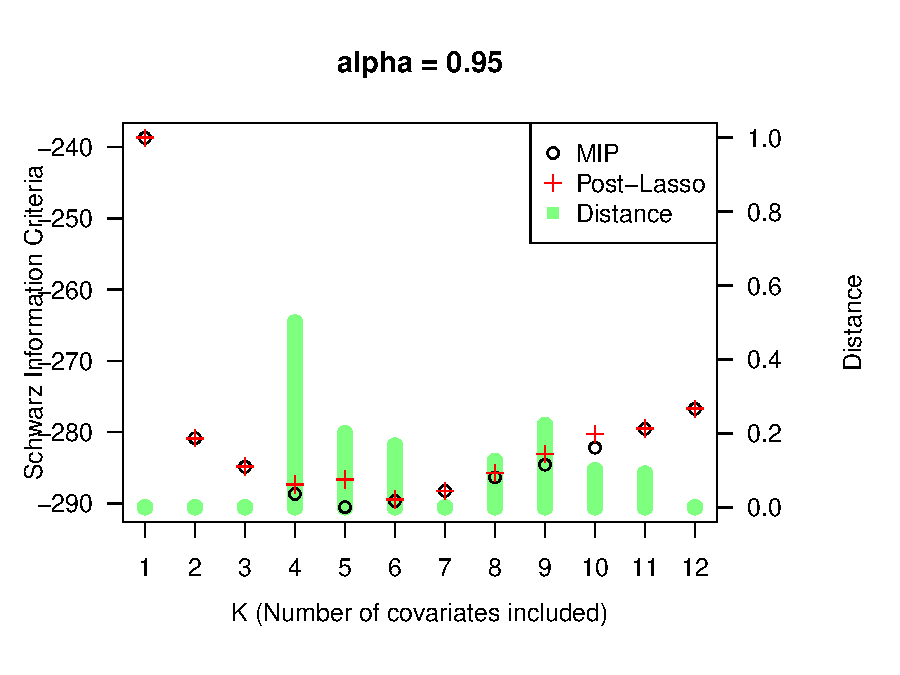
\includegraphics[width=\textwidth]{Figuras/SIC095.pdf}
			\label{fig:npqar-cross}
		\end{minipage}
	\end{minipage}
	\caption{ \textbf{REVER: Comparison of SIC values between a solution with LASSO as a variable selector and the best subset selection with MILP}. The Information Criteria is displayed on the y-axis, while the number of variables included is shown on the x-axis. Both solutions of the MILP and the best LASSO for a given $K$ are  The bars represent the distance $d$ as defined on problem (\ref{eq:metricad0})-(\ref{eq:metricad4}). \\ (*) When the distance is zero, it means that the same variables are selected from both methods for a given $K$. Thus, in these cases we have the same SIC for both of them.}
	\label{fig:comparison-lm-results}
\end{figure}

